\section{Mô hình Artificial Neural Network - ANN}
\subsection{Giới thiệu}
Phương pháp thứ ba, nhóm sử dụng mạng nơ-ron nhân tạo (ANN) để dự đoán nồng độ carbon monoxide (CO) dựa trên tập dữ liệu AirQualityUCI. Thực hiện các bước từ tiền xử lý dữ liệu, huấn luyện mô hình với thuật toán tối ưu Adam, đến đánh giá hiệu suất bằng các chỉ số hồi quy và phân loại. Phương pháp này thể hiện tiềm năng trong việc giám sát chất lượng không khí, với các cơ hội cải tiến thông qua tối ưu hóa siêu tham số hoặc sử dụng kiến trúc mạng phức tạp hơn.
\subsection{Tập dữ liệu}
Tập dữ liệu AirQualityUCI chứa 9358 mẫu dữ liệu trung bình hàng giờ từ một thiết bị cảm biến hóa học đa cảm biến được triển khai tại một thành phố ở Ý, từ tháng 3 năm 2004 đến tháng 2 năm 2005. Dữ liệu bao gồm các phản hồi từ năm cảm biến oxit kim loại và các phép đo môi trường như nhiệt độ (T), độ ẩm tương đối (RH), và độ ẩm tuyệt đối (AH). Nồng độ CO thực tế (CO(GT)) được cung cấp bởi một thiết bị phân tích được chứng nhận, đóng vai trò là biến mục tiêu. Các giá trị thiếu được đánh dấu bằng \textbf{-200}, và dữ liệu có tính chất chuỗi thời gian, đa biến.

\textbf{Các đặc trưng sử dụng:} PT08.S1(CO), NMHC(GT), C6H6(GT), nhiệt độ (T), độ ẩm tương đối (RH), độ ẩm tuyệt đối (AH), PT08.S2(NMHC), NOx(GT), PT08.S3(NOx), NO2(GT), PT08.S4(NO2), PT08.S5(O3), hour, day, month, year (chuyển đổi từ cột Date, Time).

\textbf{Biến mục tiêu:}  CO(GT).
\subsection{Tiền xử lý dữ liệu}
\begin{itemize}
    \item \textbf{Đọc dữ liệu:} Sử dụng thư viện Pandas để đọc file CSV. Dữ liệu sử dụng dấu ; phân tách các cột và ký hiệu dấu phẩy ta xử lý chuyển sang dấu chấm '.'. Loại bỏ các cột không cần thiết và chuyển đổi dữ liệu đặc trưng "Date", "Time" sang hour, day, month, year.
    \item \textbf{Xử lý giá trị thiếu:} Đối với các dữ liệu CO(GT) có giá trị \textbf{-200} ta loại bỏ dữ liệu đó, còn các dữ liệu có đặc trưng khác bị thiếu (được đánh dấu bằng \textbf{-200}) ta thay bằng giá trị trung bình của cột tương ứng.
    \item \textbf{Chuẩn hóa dữ liệu: } Sử dụng chuẩn hóa Z-score chuyển mỗi thuộc tính về giá trị có trung bình 0 và độ lệch chuẩn 1. Cụ thể, với mỗi thuộc tính $x$, tính $x' = \frac{x - \mu}{\sigma}$ (với $\mu$ là giá trị trung bình và $\sigma$ là độ lệch chuẩn của thuộc tính đó trên tập huấn luyện). Việc chuẩn hóa giúp tăng tốc độ hội tụ của mạng và tránh cho thuộc tính có phạm vi lớn lấn át các thuộc tính khác trong quá trình huấn luyện.
\end{itemize}
Sau đó chia dữ liệu thành tập huấn luyện ($80\%$) và tập kiểm tra ($20\%$).

\begin{itemize}
    \item \textbf{Số mẫu train sau khi tiền xử lý dữ liệu:} 6139
    \item \textbf{Số mẫu test sau khi tiền xử lý dữ liệu:} 1535
    \item \textbf{Số đặc trưng sau khi tiền xử lý dữ liệu:} 16
\end{itemize}

\subsection{Kiến trúc mô hình Artificial Neural Network}
\subsubsection{Kiến trúc Mạng Nơ - ron}
Mô hình sử dụng một mạng nơ-ron truyền thẳng với cấu trúc sau:
\begin{itemize}
    \item \textbf{Tầng đầu vào:} Số nơ-ron tương ứng với số đặc trưng là 16
    \item \textbf{Tầng ẩn (hidden\_size):} 64 nơ-ron với hàm kích hoạt ReLU (Rectified Linear Unit), giúp mô hình học các mối quan hệ phi tuyến
    \item \textbf{Tầng đầu ra:} Một nơ-ron với kích hoạt tuyến tính, phù hợp cho bài toán hồi quy
\end{itemize}

\subsubsection{Cấu hình huấn luyện}
Quá trình huấn luyện mô hình được thiết lập với các siêu tham số như sau:
\begin{itemize}
    \item \textbf{Số epoch:} 3000 epoch
    \item \textbf{Batch size:} 32
    \item \textbf{Tốc độ học (learning rate):} 0.001 (Giá trị learning rate nhỏ giúp Adam cập nhật trọng số một cách từ tốn, giảm nguy cơ nhảy quá đà qua cực trị của hàm mất mát)
    \item \textbf{Random\_state}: 42 để đảm bảo khả năng tái lập kết quả
\end{itemize}

Quá trình huấn luyện sử dụng khởi tạo trọng số ngẫu nhiên theo phân phối đều và giám sát mất mát sau mỗi \textbf{300} epoch để đánh giá sự hội tụ.

\subsection{Kết quả và đánh giá}
\subsubsection{Đánh giá trên tập kiểm thử}
\subsubsubsection{Hiệu suất hồi quy}
\begin{itemize}
    \item \textbf{Mean Squared Error (MSE):} 0.1090
    \item \textbf{Root MSE (RMSE):} 0.3302
    \item \textbf{Mean Absolute Error (MAE):} 0.2427
    \item \textbf{R\textsuperscript{2} score:} 0.9485
\end{itemize}
\subsubsubsection{Hiệu suất phân loại}
Trong nhiệm vụ phân loại nhị phân, nồng độ CO được phân loại thành cao ($\geq$ trung bình) hoặc thấp ($<$ trung bình). Mô hình đạt được:
\begin{itemize}
    \item \textbf{Accuracy:}  0.9368
    \item \textbf{Precision: } 0.9377
    \item \textbf{F1 Score:} 0.9199
\end{itemize}
\subsubsection{Quá trình huấn luyện}
Mất mát được giám sát sau mỗi \textbf{300} epoch, cho thấy xu hướng giảm dần, biểu thị sự hội tụ của mô hình. Đề xuất bao gồm một biểu đồ mất mát theo kỷ nguyên để minh họa quá trình này.

\begin{figure}[H]
    \centering
    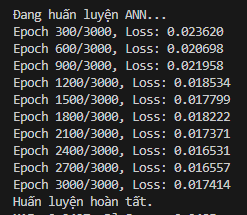
\includegraphics[width=0.7\textwidth]{images/ANN/300epoch.png}
    \caption{Mất mát được giám sát sau mỗi 300 epoch}
    \label{fig:ann}
\end{figure}

\subsubsection{Biểu đồ tầm quan trọng của đặc trưng}
So các đặc trưng khác với đặc trưng đóng góp nhiều nhất là \textbf{PT08.S1(CO)}
\begin{figure}[H]
    \centering
    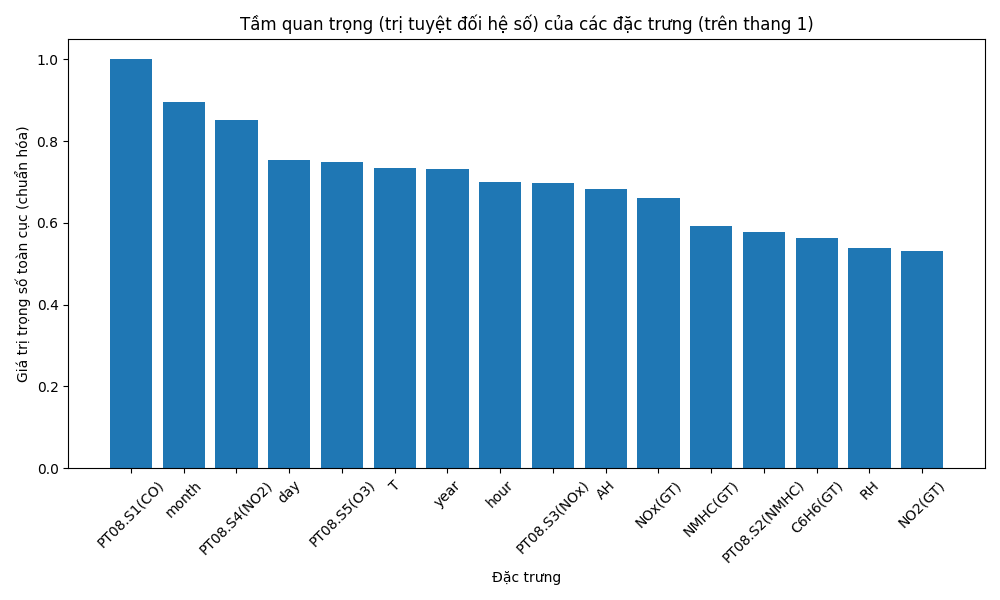
\includegraphics[width=0.8\textwidth]{images/ANN/Tamquantrongdactrung.png}
    \caption{Tầm quan trọng của các đặc trưng}
    \label{fig:ann}
\end{figure}

\subsubsection{Biểu đồ so sánh giá trị thực tế và dự đoán}
\begin{figure}[H]
    \centering
    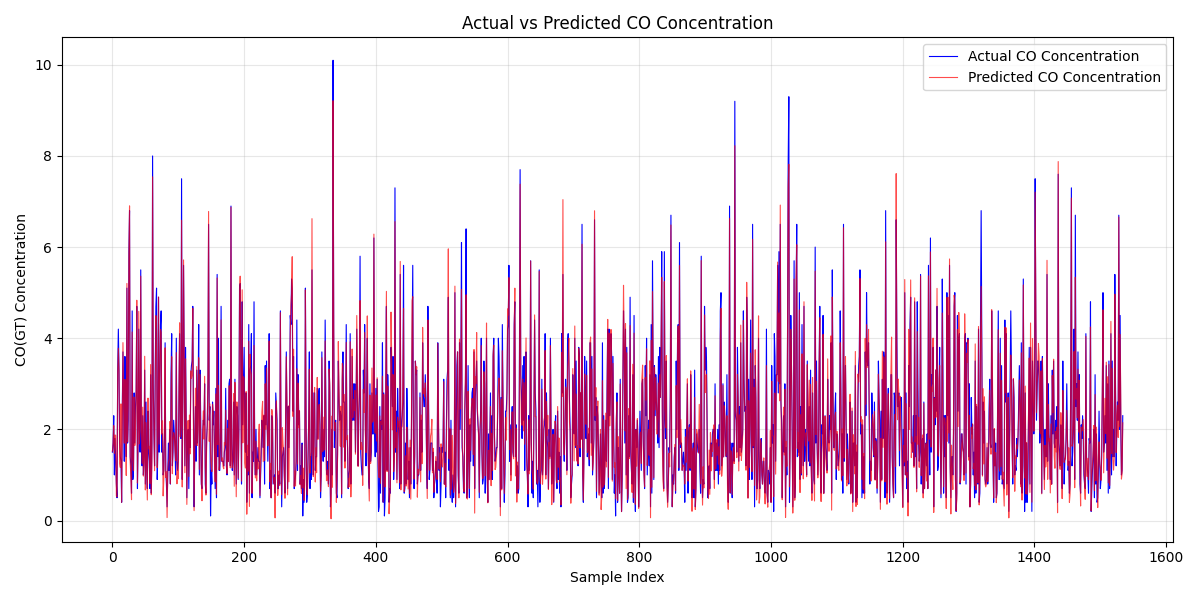
\includegraphics[width=0.8\textwidth]{images/ANN/SOkqANN.png}
    \caption{so sánh giá trị thực tế và dự đoán}
    \label{fig:ann}
\end{figure}

\subsubsection{Kết quả cuối sau khi chạy code}
\begin{figure}[H]
    \centering
    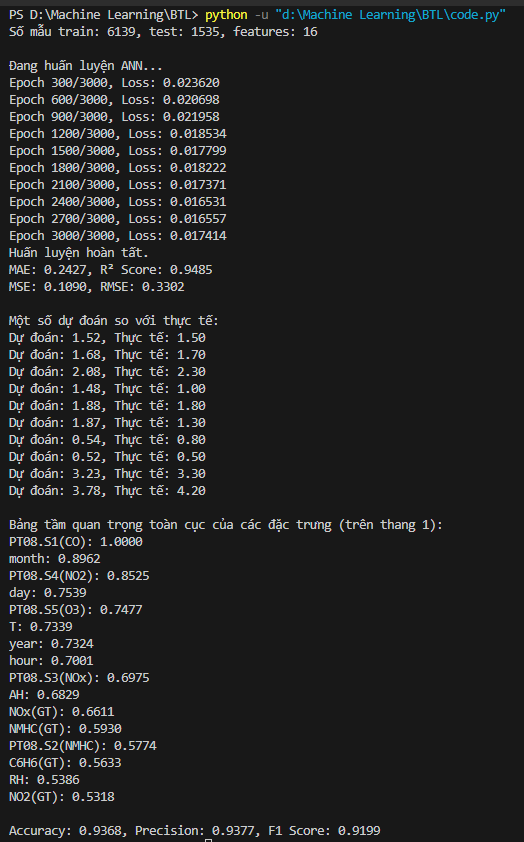
\includegraphics[width=0.7\textwidth]{images/ANN/Ketquatoanbo.png}
    \caption{Kết quả sau khi chạy code}
    \label{fig:ann}
\end{figure}

\subsection{Kết luận}
Mô hình Artificial Neural Network đã được triển khai thành công để dự đoán nồng độ CO trên tập dữ liệu AirQualityUCI. Phương pháp này tận dụng sức mạnh của học máy để xử lý dữ liệu cảm biến và môi trường, mang lại tiềm năng trong việc giám sát chất lượng không khí. Để cải thiện, có thể:
\begin{itemize}
    \item Tối ưu hóa siêu tham số (số nơ-ron, tỷ lệ học, số lớp ẩn).
    \item Thử nghiệm các kiến trúc mạng phức tạp hơn, như mạng nơ-ron hồi quy (RNN) hoặc mạng nơ-ron tích chập (CNN).
    \item Kết hợp thêm dữ liệu bên ngoài
\end{itemize}
